\subsection{Topological Connectedness and Paths}

Connectedness is an open-set obstruction to splitting a space into two visible pieces. In general topology it is most naturally phrased by separations and then transported through continuous maps.

\begin{definition} \label{def:topological-connectedness} \hlt{Connected Topological Spaces}\\
Let $(X,\tau)$ be a topological space, and let $E\subseteq X$.
\begin{enumerate}[label=(\roman*)]
\setlength{\itemsep}{0pt}
\item A set $A\subseteq X$ is \hlt{clopen} iff $A\in\tau$ and $X\setminus A\in\tau$.
\item A \hlt{separation} of $X$ is a pair $(U,V)$ with $U,V\in\tau$, $U,V\neq\emptyset$, $U\cap V=\emptyset$, and $X=U\cup V$.
\item $X$ is \hlt{connected} iff no separation of $X$ exists.
\item $E$ is \hlt{connected} iff $(E,\tau_E)$ is connected, where $\tau_E\defeq\{E\cap U:U\in\tau\}$.\\
Equivalently, $E$ is disconnected iff $\exists U,V\in\tau$ with $U\cap E\neq\emptyset$, $V\cap E\neq\emptyset$, $E\subseteq U\cup V$, and $E\cap U\cap V=\emptyset$.
\end{enumerate}
\hlt{Key Insight}: Connectedness forbids a nonempty disjoint open split.
\end{definition}

\begin{proposition} \label{prop:metric-and-topological-connectedness-agree} \hlt{Metric and Topological Connectedness Agree}\\
Let $(X,d)$ be a metric space with its metric topology, and let $E\subseteq X$.\\
Then $E$ is connected by Definition \ref{def:separated-and-connected-sets} iff it is connected as a topological subspace by Definition \ref{def:topological-connectedness}.
\begin{proof}
\begin{enumerate}[label=\roman*.]
\setlength{\itemsep}{0pt}
\item[$(\Rightarrow)$] Assume $E$ is connected in the metric sense. If $(U,V)$ separates the topological subspace $E$, then $U,V\neq\emptyset$ and $E=U\cup V$.\\
For $u\in U$, choose an open $O_u\subseteq X$ with $u\in O_u$ and $E\cap O_u\subseteq U$. Then $O_u\cap V=\emptyset$, so $u\notin\overline{V}$.\\
Hence $U\cap\overline{V}=\emptyset$, and similarly $\overline{U}\cap V=\emptyset$. Thus $U,V$ are separated in the metric sense, a contradiction.
\item[$(\Leftarrow)$] Assume $E$ is connected as a topological subspace. If nonempty $A,B\subseteq E$ are separated in the metric sense and $E=A\cup B$, then $A=E\cap(X\setminus\overline{B})$ and $B=E\cap(X\setminus\overline{A})$. Thus $A,B$ are open in $E$, so $(A,B)$ separates the topological subspace $E$, a contradiction.
\end{enumerate}
\hlt{Structural Commentary}: Ambient closures and relative open complements translate through subspace neighborhoods.\\
\hlt{Key Insight}: Each side avoids the opposite ambient closure exactly when it is relatively open.
\end{proof}
\end{proposition}

\begin{proposition} \label{prop:topological-connected-clopen-characterization} \hlt{Connectedness and Clopen Sets}\\
Let $(X,\tau)$ be a topological space. Then $X$ is connected iff $(\forall A\subseteq X)\,[A\text{ clopen}\Rightarrow(A=\emptyset\lor A=X)]$.
\begin{proof}
\begin{enumerate}[label=\roman*.]
\setlength{\itemsep}{0pt}
\item[$(\Rightarrow)$] If $A\subseteq X$ is clopen, nonempty, and proper, then $(A,X\setminus A)$ is a separation of $X$, impossible.
\item[$(\Leftarrow)$] If $(U,V)$ separates $X$, then $U=X\setminus V$ is clopen, nonempty, and proper, impossible.
\end{enumerate}
\hlt{Structural Commentary}: Complements convert separations into clopen sets.\\
\hlt{Key Insight}: Connected means no nontrivial clopen subset.
\end{proof}
\end{proposition}

\begin{proposition} \label{prop:continuous-image-connected-topological} \hlt{Continuous Images of Connected Spaces Are Connected}\\
Let $X,Y$ be topological spaces and let $f:X\to Y$ be continuous. If $X$ is connected, then $f(X)$ is connected in the subspace topology.
\begin{proof}
Let $g:X\to f(X)$ be $f$ with codomain restricted to $f(X)$. If $W$ is open in $f(X)$, choose $O$ open in $Y$ with $W=f(X)\cap O$. Then $g^{-1}(W)=f^{-1}(O)$ is open in $X$ by Proposition \ref{prop:topological-continuity-open-preimages}(i), so $g$ is continuous.\\
If $(U,V)$ separates $f(X)$, then $g^{-1}(U)$, $g^{-1}(V)$ are nonempty disjoint open subsets of $X$ with union $X$, contrary to connectedness of $X$.\\
\hlt{Structural Commentary}: Restrict the codomain to make the image map surjective.\\
\hlt{Key Insight}: Separations pull back by continuity.
\end{proof}
\end{proposition}

\begin{definition} \label{def:topological-intermediate-value-property} \hlt{Intermediate Value Property}\\
A topological space $X$ has the \hlt{intermediate value property} iff $(\forall f:X\to\R)\,[f\text{ continuous}\Rightarrow f(X)\text{ is an interval}]$.
\end{definition}

\begin{theorem} \label{thm:topological-connected-iff-ivp} \hlt{Connectedness and the Intermediate Value Property}\\
Let $X$ be a topological space. Then $X$ is connected iff $X$ has the intermediate value property.
\begin{proof}
\begin{enumerate}[label=\roman*.]
\setlength{\itemsep}{0pt}
\item[$(\Rightarrow)$] If $f:X\to\R$ is continuous, then $f(X)$ is topologically connected by Proposition \ref{prop:continuous-image-connected-topological} and connected in the metric sense by Proposition \ref{prop:metric-and-topological-connectedness-agree}. Hence $f(X)$ is an interval by Theorem \ref{thm:connected-subsets-of-real-line-interval-property}.
\item[$(\Leftarrow)$] We prove the contrapositive. If $(U,V)$ separates $X$, define $f:X\to\R$ by $f|_U=0$ and $f|_V=1$.\\
For an open $O\subseteq\R$, $f^{-1}(O)\in\{\emptyset,U,V,X\}$, so $f$ is continuous by Proposition \ref{prop:topological-continuity-open-preimages}(i). However, $f(X)=\{0,1\}$ is not an interval.
\end{enumerate}
\hlt{Structural Commentary}: Separations produce continuous two-valued tests.\\
\hlt{Key Insight}: Intermediate values are connectedness seen by $\R$.
\end{proof}
\end{theorem}

\begin{proposition} \label{prop:connected-union-common-point} \hlt{Unions Through a Common Point}\\
Let $\{C_\alpha\}_{\alpha\in A}$ be connected subsets of a topological space $X$ with $\bigcap\limits_{\alpha\in A}C_\alpha\neq\emptyset$. Then $C\defeq\bigcup\limits_{\alpha\in A}C_\alpha$ is connected.
\begin{proof}
If $A=\emptyset$, then $C=\emptyset$ is connected. Assume $A\neq\emptyset$ and choose $p\in\bigcap\limits_{\alpha\in A}C_\alpha$.\\
Suppose $(U,V)$ separates $C$ and, after interchanging the sides if necessary, $p\in U$.\\
For $\alpha\in A$, the pair $(U\cap C_\alpha,V\cap C_\alpha)$ would separate $C_\alpha$ if $C_\alpha\cap V\neq\emptyset$.\\
Hence $(\forall\alpha\in A)\,C_\alpha\cap V=\emptyset$, so $V\cap C=\emptyset$, contrary to the nonemptiness of $V$.\\
\hlt{Structural Commentary}: Each connected piece must stay on the side containing the shared point.\\
\hlt{Key Insight}: A common point blocks separation.
\end{proof}
\end{proposition}

\begin{proposition} \label{prop:connected-closure-sandwich} \hlt{Connectedness Between a Set and Its Closure}\\
Let $(X,\tau)$ be a topological space and let $A\subseteq B\subseteq\overline{A}$. If $A$ is connected, then:
\begin{enumerate}[label=(\roman*)]
\setlength{\itemsep}{0pt}
\item $B$ is connected;
\item $\overline{A}$ is connected.
\end{enumerate}
\begin{proof}
\begin{enumerate}[label=(\roman*)]
\setlength{\itemsep}{0pt}
\item Suppose $(P,Q)$ separates $B$. Since $A$ is connected, $A\subseteq P$ or $A\subseteq Q$; assume $A\subseteq P$.\\
If $q\in Q$, choose $O\in\tau$ with $q\in O$ and $O\cap B\subseteq Q$.\\
Since $q\in B\subseteq\overline{A}$, $O\cap A\neq\emptyset$, contradicting $A\subseteq P$ and $P\cap Q=\emptyset$. Thus $Q=\emptyset$, contrary to the definition of a separation.
\item The set $\overline{A}$ is connected by (i) with $B=\overline{A}$.
\end{enumerate}
\hlt{Structural Commentary}: Relative open separation near $\overline{A}$ must meet the connected core $A$.\\
\hlt{Key Insight}: Adding only closure points cannot create a new component.
\end{proof}
\end{proposition}

\begin{definition} \label{def:topological-path-connected} \hlt{Path-Connected Spaces}\\
A topological space $X$ is \hlt{path-connected} iff $(\forall u,v\in X)(\exists\gamma:[0,1]\to X)\,[\gamma\text{ continuous}\land\gamma(0)=u\land\gamma(1)=v]$.
\end{definition}

\begin{theorem} \label{thm:path-connected-implies-connected-topological} \hlt{Path-Connected Spaces Are Connected}\\
Let $X$ be path-connected. Then $X$ is connected.
\begin{proof}
Suppose $(U,V)$ separates $X$. Choose $u\in U$, $v\in V$, and a path $\gamma:[0,1]\to X$ from $u$ to $v$.\\
The interval $[0,1]$ is connected in the metric sense by Theorem \ref{thm:connected-subsets-of-real-line-interval-property} and topologically connected by Proposition \ref{prop:metric-and-topological-connectedness-agree}.\\
Hence $\gamma([0,1])$ is connected by Proposition \ref{prop:continuous-image-connected-topological}. However, $(U\cap\gamma([0,1]),V\cap\gamma([0,1]))$ separates it, a contradiction.\\
\hlt{Structural Commentary}: A path imports interval connectedness into $X$.\\
\hlt{Key Insight}: Paths cannot cross a separation.
\end{proof}
\end{theorem}

\begin{proposition} \label{prop:connected-open-euclidean-path-connected} \hlt{Connected Open Sets in Euclidean Space Are Path-Connected}\\
Let $n\in\N$, and let $O\subseteq\R^n$ be open and connected. Then any $x,y\in O$ can be joined in $O$ by a finite polygonal path.
\begin{proof}
Fix $x_0\in O$. Write $a\sim b$ if $a,b\in O$ are joined in $O$ by a finite polygonal path.\\
Constant paths, path reversal, and concatenation make $\sim$ an equivalence relation. Set $C\defeq\{x\in O:x_0\sim x\}$.\\
Then $x_0\in C$. Let $x\in O$ and choose $r>0$ with $B(x,r)\subseteq O$. Any two points of $B(x,r)$ are joined by a segment.\\
Thus $x\in C$ implies $B(x,r)\subseteq C$. If $x\notin C$ and $B(x,r)\cap C\neq\emptyset$, a segment from a point of $C$ to $x$ would imply $x\in C$.\\
Hence $B(x,r)\cap C=\emptyset$. Therefore $C$ and $O\setminus C$ are open in $O$. Since $C\neq\emptyset$, one has $C=O$ by Proposition \ref{prop:topological-connected-clopen-characterization}.\\
Thus all points of $O$ lie in one $\sim$-equivalence class, so any two are joined by a finite polygonal path.\\
\hlt{Structural Commentary}: Polygonal reachability is both open and closed in an open set.\\
\hlt{Key Insight}: Local line segments make one component all of $O$.
\end{proof}
\end{proposition}

\begin{counterexample} \label{cex:topologist-sine-curve-connected-not-path-connected} \hlt{Connected Need Not Mean Path-Connected}\\
The converse of Theorem \ref{thm:path-connected-implies-connected-topological} fails.\\
Let $G\defeq\{(x,\sin(1/x)):0<x\leq1\}$, $L\defeq\{0\}\times[-1,1]$, and $T\defeq G\cup L\subseteq\R^2$.
\begin{enumerate}[label=(\roman*)]
\setlength{\itemsep}{0pt}
\item $T$ is connected.
\item $T$ is not path-connected.
\end{enumerate}
\begin{proof}
\begin{enumerate}[label=(\roman*)]
\setlength{\itemsep}{0pt}
\item The interval $(0,1]$ is connected in the metric sense by Theorem \ref{thm:connected-subsets-of-real-line-interval-property} and topologically connected by Proposition \ref{prop:metric-and-topological-connectedness-agree}.\\
Map $h:(0,1]\to\R^2$, $h(x)\defeq(x,\sin(1/x))$, is continuous in metric sense, hence in topological sense by Corollary \ref{cor:metric-and-topological-continuity-agree}.\\
Thus $G=h((0,1])$ is connected by Proposition \ref{prop:continuous-image-connected-topological}. For $y\in[-1,1]$, choose $\theta\in[-\frac{\pi}{2},\frac{\pi}{2}]$ with $\sin\theta=y$ and set $x_n\defeq\frac{1}{2\pi n+\theta}$.\\
Then $(x_n,y)=h(x_n)\to(0,y)$, so $L\subseteq\overline{G}$ by Proposition \ref{prop:sequential-closure-criterion}. Hence $T\subseteq\overline{G}$.\\
Conversely, fix $p=(x,y)\in\overline{G}$ and choose $(x_n,y_n)\subseteq G$ with $(x_n,y_n)\to p$ by Proposition \ref{prop:sequential-closure-criterion}.\\
Then $x_n\to x$, $y_n\to y$ by Theorem \ref{thm:rk-sequence-coordinate-convergence}(i). Since $(x_n)\subseteq(0,1]$, $(y_n)\subseteq[-1,1]$, then $x\in[0,1]$, $y\in[-1,1]$ by Theorem \ref{thm:closed-sets-and-limit-points-via-sequences}(ii).\\
If $x=0$, then $p\in L$. If $x>0$, then $h(x_n)\to h(x)$ by Theorem \ref{thm:metric-continuity-sequential-characterization}; hence $p=h(x)\in G$ by Theorem \ref{thm:metric-sequence-basic-properties}(ii).\\
Thus $\overline{G}\subseteq T$, so $T=\overline{G}$ and $T$ is connected by Proposition \ref{prop:connected-closure-sandwich}(ii).
\item Suppose $T$ is path-connected. Choose a path $\gamma:[0,1]\to T$ from $(0,0)$ to $(1,\sin1)$ and write $\gamma(t)=(a(t),b(t))$.\\
The coordinate maps $a,b$ are topologically continuous by Proposition \ref{prop:product-topology-coordinate-continuity} and metrically continuous by Corollary \ref{cor:metric-and-topological-continuity-agree}.\\
Set $Z\defeq\{t\in[0,1]:a(t)=0\}$. Since $[0,1]\setminus Z=a^{-1}(\R\setminus\{0\})$ is open by Proposition \ref{prop:topological-continuity-open-preimages}(i), $Z$ is nonempty and closed in $[0,1]$.\\
Interval $[0,1]$ is compact in its usual topology by Theorem \ref{thm:heine-borel-rk},  Proposition \ref{prop:compact-subspace-ambient-cover-equivalence}; hence $Z$ is compact by Proposition \ref{prop:closed-subsets-compact-topological}.\\
The identity on $Z$ attains its maximum $t_0$ by Corollary \ref{cor:extreme-value-compact-topological}. Since $a(1)=1$, one has $t_0<1$.\\
One has $(\forall t\in(t_0,1])\,a(t)>0$ by $a([0,1])\subseteq[0,1]$ and maximality of $t_0$. Set $t_j\defeq t_0+\frac{1-t_0}{j+1}$.\\
For $j\in\N$, choose $N_j\in\N$ so large that $s_j^+\defeq\frac{1}{\pi/2+2\pi N_j}<a(t_j)$ and $s_j^-\defeq\frac{1}{3\pi/2+2\pi N_j}<a(t_j)$ by Theorem \ref{thm:archimedean-and-rational-density}(i).\\
By Theorem \ref{thm:intermediate-value-theorem}, there are $u_j^+,u_j^-\in(t_0,t_j)$ with $a(u_j^\pm)=s_j^\pm$. Since $u_j^\pm>t_0$, $\gamma(u_j^\pm)\in G$, so $b(u_j^+)=1$ and $b(u_j^-)=-1$.\\
Convergence $\frac{1-t_0}{j+1}\to0$ follows by Theorem \ref{thm:special-sequence-limits}(i), Proposition \ref{prop:subsequences-of-convergent-sequences}(i), Theorem \ref{thm:complex-sequence-limit-algebra}(ii), so $t_j\to t_0$ by Theorem \ref{thm:complex-sequence-limit-algebra}(ii).\\
Hence $u_j^\pm\to t_0$ by Theorem \ref{thm:pinching-theorem-sequences} with $t_0<u_j^\pm<t_j$. Thus $b(u_j^\pm)\to b(t_0)$ by Theorem \ref{thm:metric-continuity-sequential-characterization}.\\
Since $b(u_j^+)=1$, $b(u_j^-)=-1$, uniqueness of real sequence limits by Proposition \ref{prop:convergent-sequence-basic-consequences}(i) forces $b(t_0)=1$, $b(t_0)=-1$, contradiction.
\end{enumerate}
\hlt{Structural Commentary}: Closure transfers connectedness from $G$, while the last zero forces incompatible vertical limits.\\
\hlt{Key Insight}: Infinite oscillation near $x=0$ prevents a path from leaving $L$.
\end{proof}
\end{counterexample}

\noindent Figure \ref{fig:topologist-sine-curve-connected-not-path} plots the oscillatory graph $G$ approaching the vertical segment $L$, the accumulation geometry behind the distinction between connectedness and path-connectedness.

\begin{visualizationfigure}[H]
  \centering
  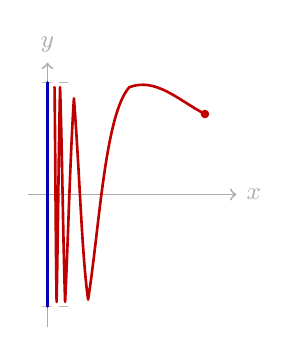
\begin{tikzpicture}[
  x=2.0cm,
  y=1.42cm,
  every node/.style={font=\small},
  line cap=round,
  line join=round,
  axis/.style={->, gray!65, line width=0.65pt},
  guide/.style={gray!55, dashed, line width=0.5pt},
  limit/.style={blue!70!black, line width=1.2pt},
  graph/.style={red!75!black, line width=0.95pt},
  point/.style={circle, fill=red!75!black, inner sep=1.1pt}
]
  \draw[axis] (-0.12,0) -- (1.20,0) node[right] {$x$};
  \draw[axis] (0,-1.18) -- (0,1.18) node[above] {$y$};

  \draw[guide] (-0.03,1) -- (0.18,1);
  \draw[guide] (-0.03,-1) -- (0.18,-1);

  \draw[limit] (0,-1) -- (0,1);

  \draw[graph]
    (0.045,0.96)
      .. controls (0.050,0.35) and (0.052,-0.38) .. (0.058,-0.96)
      .. controls (0.067,-0.32) and (0.071,0.38) .. (0.080,0.96)
      .. controls (0.094,0.35) and (0.098,-0.35) .. (0.112,-0.96)
      .. controls (0.132,-0.38) and (0.142,0.28) .. (0.168,0.86)
      .. controls (0.205,0.18) and (0.218,-0.54) .. (0.258,-0.94)
      .. controls (0.330,-0.30) and (0.365,0.72) .. (0.520,0.96)
      .. controls (0.690,1.05) and (0.835,0.84) .. (1.000,0.72);
  \node[point] at (1.000,0.72) {};
\end{tikzpicture}

  \caption{Topologist's sine curve: \textcolor{red!75!black}{$y=\sin(1/x)$} accumulates on \textcolor{blue!70!black}{$\{0\}\times[-1,1]$}; connected, not path-connected.}
  \label{fig:topologist-sine-curve-connected-not-path}
\end{visualizationfigure}
